\documentclass[french,a4paper]{article}
\setcounter{tocdepth}{4}
\setcounter{secnumdepth}{4}
\usepackage{float}
\usepackage{graphicx}
\newcommand{\tabitem}{\textbullet~~}
\usepackage{multirow}
\graphicspath{{img/}}
\title{PPII}
\usepackage[bottom=2.5cm,top=2.5cm,left=2.5cm,right=2.5cm]{geometry}
\author{Noé Steiner - Alexis Marcel - Lucas Laurent - Mathias Aurand-Augier}
\date{Octobre 2022}
\begin{document}

\maketitle
\newpage
\tableofcontents
\newpage
\section{Contexte du projet}
Ce rapport rend compte du Projet Pluridisciplinaire d’Informatique Intégrative dans le cadre de la première année du cycle ingénieur à TELECOM Nancy.
L’objectif de ce projet est de concevoir une application dédiée à l’optimisation des ressources dans les vergers et potagers partagés du territoire.

\newpage
\section{Etat de l'art}
\subsection{Introduction}
Les enjeux climatiques n’ont jamais été aussi élevés. Notre planète arrive à la fin de ses énergies fossiles. Les ressources deviennent rares, les changements climatiques provoquent des pénuries, des sécheresses et des catastrophes naturelles. Le mode de vie que nous connaissons aujourd’hui doit changer et devenir plus écoresponsable. L’objectif est de changer les habitudes de consommation de produits venants du monde entier en se restreignant à une zone géographique bien plus petite. La politique actuelle serait de privilégier les produits de notre pays mais essayons d’aller plus loin…

En effet, un mode de vie plus judicieux écologiquement serait de revenir à des productions locales en passant directement par les producteurs. Certaines personnes ont une surface de production( jardin, verger) mais n’ont pas le temps ou les moyens de s’en occuper. Tandis que d’autres personnes, n’ont pas de terrain mais sont prêtes à donner de leur temps pour pouvoir consommer localement.

Notre solution : utiliser les technologies modernes du web pour proposer une application permettant à n’importe qui de créer/rejoindre un jardin mais surtout de pouvoir gérer facilement un jardin sur lequel vont agir plusieurs personnes.

\subsection{Définition d’un circuit court et d’un jardin partagé}
\subsubsection{Qu’est ce qu’un circuit court ?}

Le circuit court est une pratique de commercialisation des produits agricoles consistant à limiter au maximum le nombre d’intermédiaires (en général 0 ou 1) entre le producteur et le consommateur. Il établit donc une proximité à la fois géographique et relationnelle entre le producteur et le consommateur.

Si aucun intermédiaire n’existe, on parle alors de vente directe. Elle permet notamment à l’agriculteur de mener son activité en toute indépendance, de fixer les prix qu’il désire sans laisser de commission à un quelconque intermédiaire.

Dans l’optique de vendre leurs produits, les agriculteurs d’une même région peuvent créer un partenariat de type AMAP (Association pour le Maintien de l'Agriculture Paysanne) basé sur un système de distribution de paniers  composés des produits de la ferme (éventuellement fromage, viande, légume, fruit, oeuf) et ainsi offrir une diversité importante de produit de saison. Ils peuvent également utiliser d'autres réseaux tels que la Ruche qui Dit Oui, ou encore Bienvenue à la ferme. Mais il existe également d’autres alternatives de vente tels que les drives fermiers qui consistent pour les agriculteurs à proposer leurs produits fermiers en ligne, avec le retrait de la commande dans un point de retrait. Il peut également vendre ses produits par l’intermédiaire de coopératives ou de magasins bio (directement en contact avec le producteur) ou simplement stand dans les marchés du dimanche.

Durant le printemps 2020 et le confinement, les producteurs ont été de plus en plus nombreux à vendre en circuits courts. Malgré cela, la vente directe ne représente aujourd’hui que 5 à 10\% de la consommation alimentaire totale en France.
\subsubsection{Qu’est ce qu’un jardin partagé ?}
\textbf{Un jardin partagé est un jardin conçu, construit et cultivé collectivement par les habitants d’un quartier.} Le but étant que chaque membre du jardin participe quotidiennement à sa gestion.

L’émergence des jardins partagés remonte au 19ème siècle lors de la révolution industrielle. En effet, les populations essentiellement rurales se sont dirigées vers les villes pour trouver du travail. Cependant, les conditions de vie étaient précaires et les jardins partagés appelés  “jardins ouvriers” étaient un moyen de survie. De ce fait, lors de la première guerre mondiale, les jardins partagés ont connu un essor conséquent du fait des conditions précaires, du manque de nourriture.  Dans les années 1970, suite au développement économique, les jardins partagés connaissent un déclin majeur, la population n'en éprouvant plus le besoin.

Cependant, au fil le temps, le développement de la mondialisation a favorisé l’importation au détriment de la production à l’échelle locale. Les produits importés ont ainsi pris de plus en plus de place dans les rayons de nos grandes surfaces. La plupart des français ont ainsi recommencé à privilégier les circuits courts tels que les jardins partagés.

La création de jardin partagé repose aujourd’hui sur l’initiative des habitants. C’est un projet de quartier. La notion de “jardin partagé” est cependant à distinguer de celle de “jardin familial”.  Un jardin familial est un terrain divisé en parcelles. Chaque habitant dispose de sa propre parcelle qu’il cultive individuellement.

Il existe également une autre manière d’exploiter le concept de jardin partagé : le co-jardinage. En effet, si une personne dispose d’un jardin qu’elle n’exploite pas, elle peut le prêter à une personne qui rêve de faire du jardinage. Il s’agit ici un échange gagnant-gagnant basé sur la confiance, la convivialité, et l'entraide entre le propriétaire du jardin et le jardinier. Le propriétaire prête gracieusement un bout de son jardin, et en échange, le jardinier fait profiter d'une partie de ses récoltes.

En 2021, le gouvernement a lancé un appel aux projets de jardins partagés dans le cadre du programme France Relance. Par cet appel, le gouvernement propose des aides financières aux organismes voulant mettre en place des jardins partagés. De nombreux projets de jardins partagés ont déjà été mis en place grâce à cet appel.
\begin{figure}[H]
    \centering
    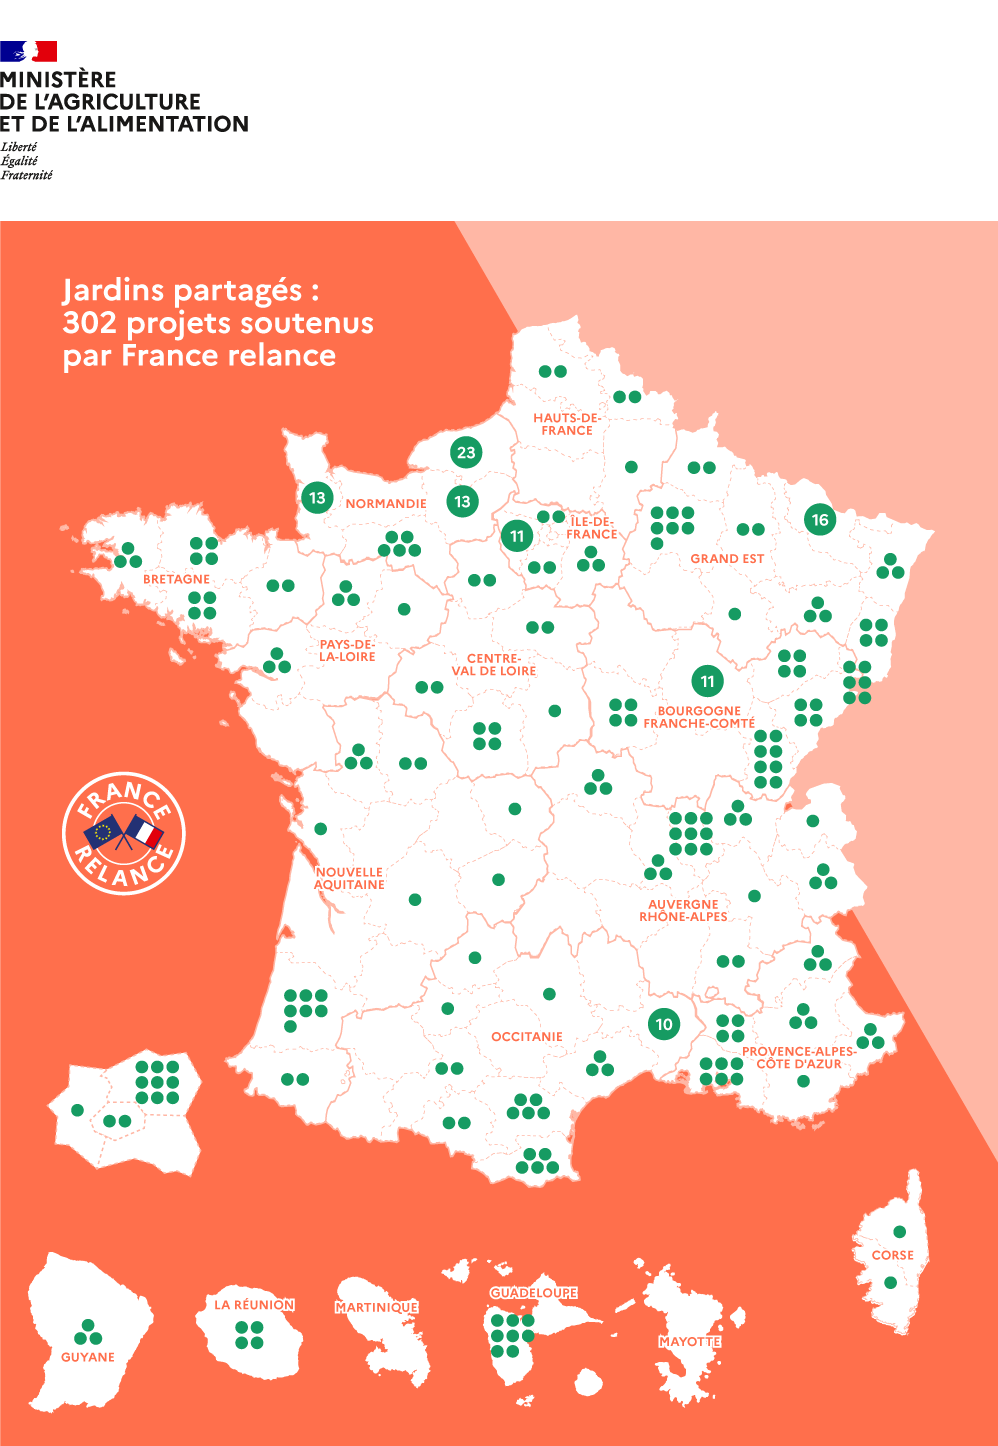
\includegraphics[width=0.5\textwidth]{img/francerelance_carte.png}
    \caption{Jardins partagés en France}
\end{figure}
Le concept de jardin partagé est aujourd’hui en développement et la population s’investit de plus en plus dans une démarche de consommation en circuit court. Le but de ce projet est ainsi de développer une application permettant la gestion d’un jardin partagé.

C’est pourquoi notre projet s’inscrit précisément dans la tendance actuelle en favorisant les circuits courts et en permettant à des personnes de faire le pas dans le monde des jardins partagés.
\subsection{Les jardins partagés et les technologies}
La plupart des applications déjà existantes permettent en général soient : de gérer son propre jardin, soit de créer ou rejoindre des jardins partagés mais peu d’application ne propose d’aide pour le gérer (planning, todo list des taches à faire dans le jardin).

Nous avons ainsi répertorié plusieurs applications existente sur le sujet. Nous avons classé leurs fonctionnalités principales dans un tableau :

\begin{center}
    \begin{tabular}{ |l| p{3cm} | p{3cm} | p{3cm} | p{3cm} | }
        \hline
                         & \raggedright création de jardin public(visible sur la carte) & \raggedright Création de jardin privée ( disponible sur lien d’invitation) & \raggedright Gestion globale du jardin & Gestion précise du jardin en organisation de tâche par parcelle \\
        \hline
        Groww            &                                                              &                                                                            & x                                      &                                                                 \\
        \hline
        AdopteMaTomate   & x                                                            &                                                                            &                                        &                                                                 \\
        \hline
        Pandasuite       & x                                                            &                                                                            &                                        &                                                                 \\
        \hline
        Plantezcheznous  & x                                                            &                                                                            &                                        &                                                                 \\
        \hline
        Click and garden & x                                                            &                                                                            &                                        &                                                                 \\

        \hline
    \end{tabular}
\end{center}

Groww est une application de gestion de jardin qui permet d’avoir une liste de tâches à faire en fonction de ses plantes. Cependant, ce logiciel est limité pour la gestion d’un jardin entier séparé en plusieurs parties et surtout il ne permet pas de gérer plusieurs contributeurs au jardin.

Les autres applications centrées sur le principe de jardin partagé permettent seulement de créer un jardin qui sera affiché sur une carte à l’adresse du jardin. N’importe qui peut alors faire une demande pour rejoindre le jardin en cliquant directement sur la carte. Cependant ces applications n’incluent pas la gestion du jardin, ce qui peut être très complexe à partir du moment où le jardin est partagé avec plusieurs personnes.

C’est pourquoi notre application permettra non seulement de créer et de rejoindre des jardins mais comprendra la gestion détaillée du jardin. De plus, créer un jardin n’engendrera pas forcément un point sur la carte à l’adresse du jardin (jardin public). En effet, un jardin pourra être privé et les utilisateurs pourront rejoindre le jardin seulement grâce à un lien d’invitation envoyé par le créateur du jardin.


\newpage
\section{Gestion de projet}
\subsection{Équipe de projet}
Ce projet est un projet local réalisé en groupe de 4 personnes :
\begin{itemize}
    \item Alexis MARCEL
    \item Lucas LAURENT
    \item Noé STEINER
    \item Mathias AURAND-AUGIER
\end{itemize}
Le comité de pilotage est constitué de :
\begin{itemize}
    \item Anne-Claire HEURTEL
    \item Olivier FESTOR
    \item Gérald OSTER
\end{itemize}
Ces personnes constituent les parties prenantes de notre projet ainsi que les acteurs influents sur le livrables :
\begin{figure}[H]
    \centering
    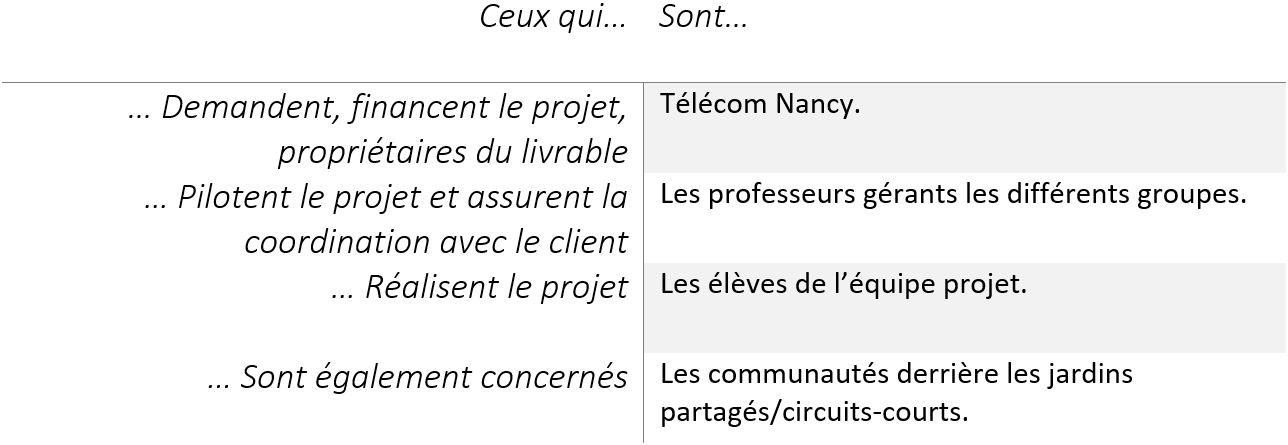
\includegraphics[width=0.75\textwidth]{img/parties_prenantes.png}
    \caption{Parties prenantes}
\end{figure} 
\subsection{Organisation au sein de l’équipe projet}
Nous avons réalisé plusieurs réunions en présentiel dans les locaux de Télécom Nancy mais également sur Discord. Ces réunions nous ont permis de mettre en commun nos avancés régulièrement, de partager nos connaissances sur des problématiques et de nous organiser de manière optimale.

De plus, dès le début de notre projet nous avons mis en place un projet Trello. Trello est une application permettant d’organiser facilement un projet en reposant sur une organisation en planches listant des cartes, chacune représentant des tâches. Ces tâches peuvent ensuite être déplacées permettant de découper notre projet en plusieurs jalons dynamiquement.

Les comptes rendus des réunions réalisés sont présents dans l’Annexe 1.

Enfin pour partager notre code, nous avons utilisé GitLab.

Ce rapport a été rédigé en \LaTeX.

\subsection{Triangle qualité-cout-délai}
Afin d’établir des objectifs cohérents, et réalisables dans les délais, nous avons réalisé le triangle qualité-coût-délai (mettre le triangle). On remarque ainsi, les délais étant relativement courts, que nous avons tout intérêt à se fixer des objectifs pas trop ambitieux sous peine de renoncer à certaines fonctionnalités faute de temps. 

\begin{figure}[H]
    \centering
    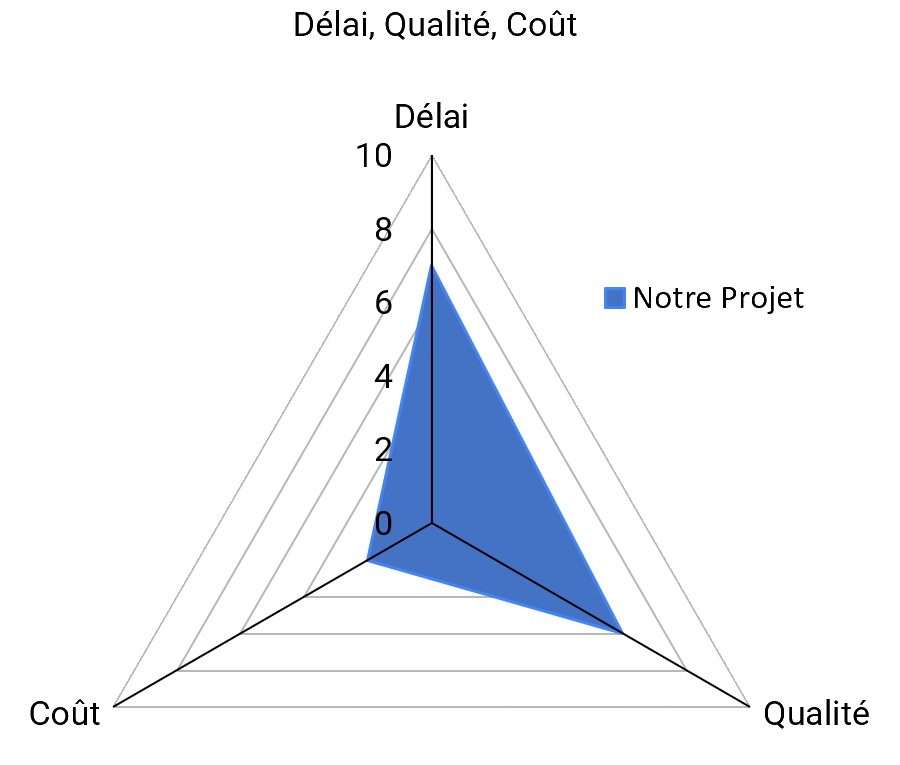
\includegraphics[width=0.5\textwidth]{img/triangle_QCD.png}
    \caption{Triangle DQC}
\end{figure} 

\subsection{Matrice SWOT}
Afin d’avoir une vision plus globale de nos ressources et des facteurs interne et externe agissant sur le projet, nous avons ensuite réalisé la matrice SWOT de notre projet.

\begin{figure}[H]
    \centering
    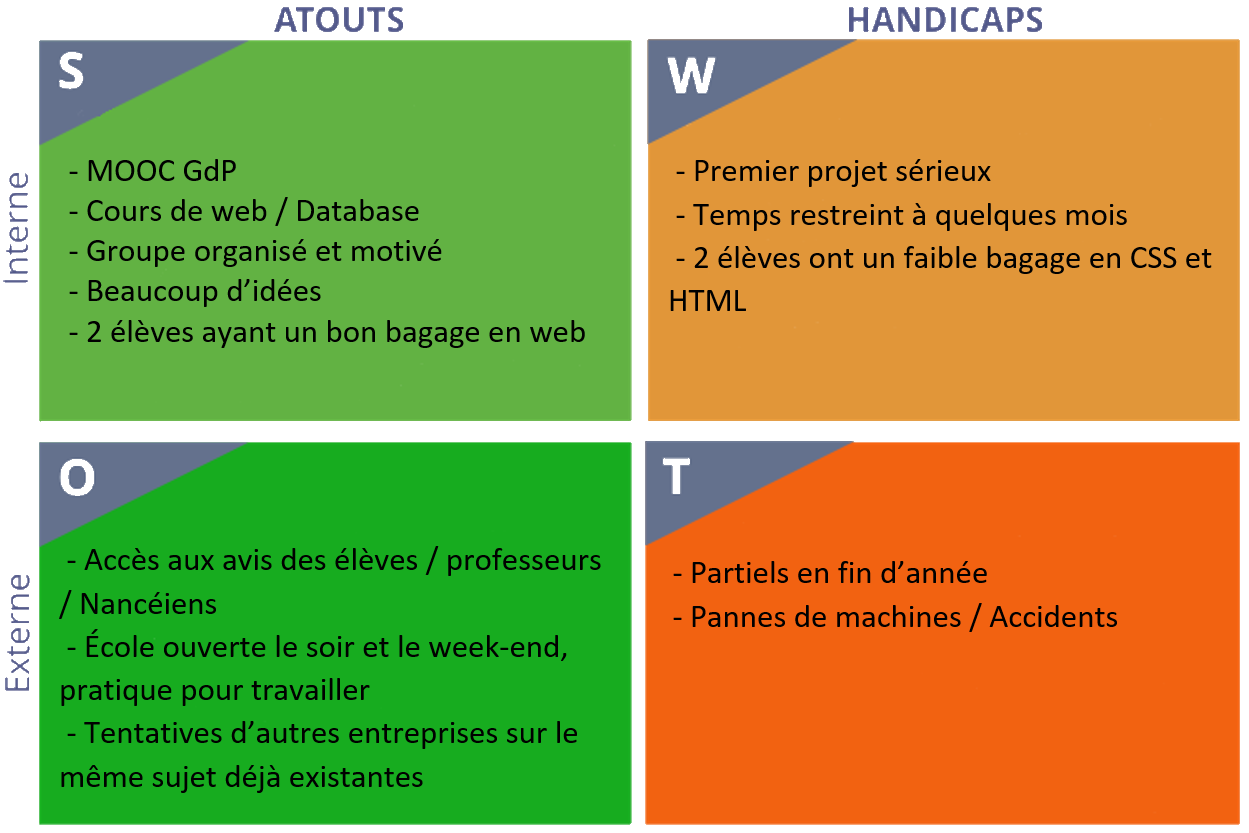
\includegraphics[width=0.75\textwidth]{img/SWOT.png}
    \caption{Matrice SWOT}
\end{figure} 

On a ainsi remarqué que notre projet présentait de nombreux points fort notamment grâce aux connaissances acquises grâce aux cours de Télécom Nancy et à l’expérience forte de deux des membres de l’équipe projet.  Cependant, plusieurs facteurs internes constituent nos faiblesses notamment les courts délais du projet qui nous obligeront à être concis et efficaces dans notre travail, ou encore le faible bagage informatique de deux des membres de l’équipe. Néanmoins, ces lacunes constituent pour eux l’opportunité d’apprendre, et de progresser avec l’aide des membres expérimentés de l’équipe.

\subsection{Profil de projet}
Afin d’avoir une vision plus globale sur notre projet, nous avons également réalisé le profil du projet (le budget étant égal à 0, nous avons choisi de ne pas le représenter dans notre profil). On remarque ainsi du fait des nombreuses fonctionnalités que nous avons l’intention d’implémenter dans notre application que notre projet est plutôt de taille moyenne et de complexité élevée bien que les enjeux soient peu importants (en dehors de la note finale qui compte dans notre moyenne). Au vu de l’état de l’art établi, l’innovation du projet semble assez importante puisque nous avons choisi de compiler différentes fonctionnalités de plusieurs applications en une et d’en rajouter de nouvelles si possibles. Par ailleurs, les délais du projet sont relativement courts.
\begin{figure}[H]
    \centering
    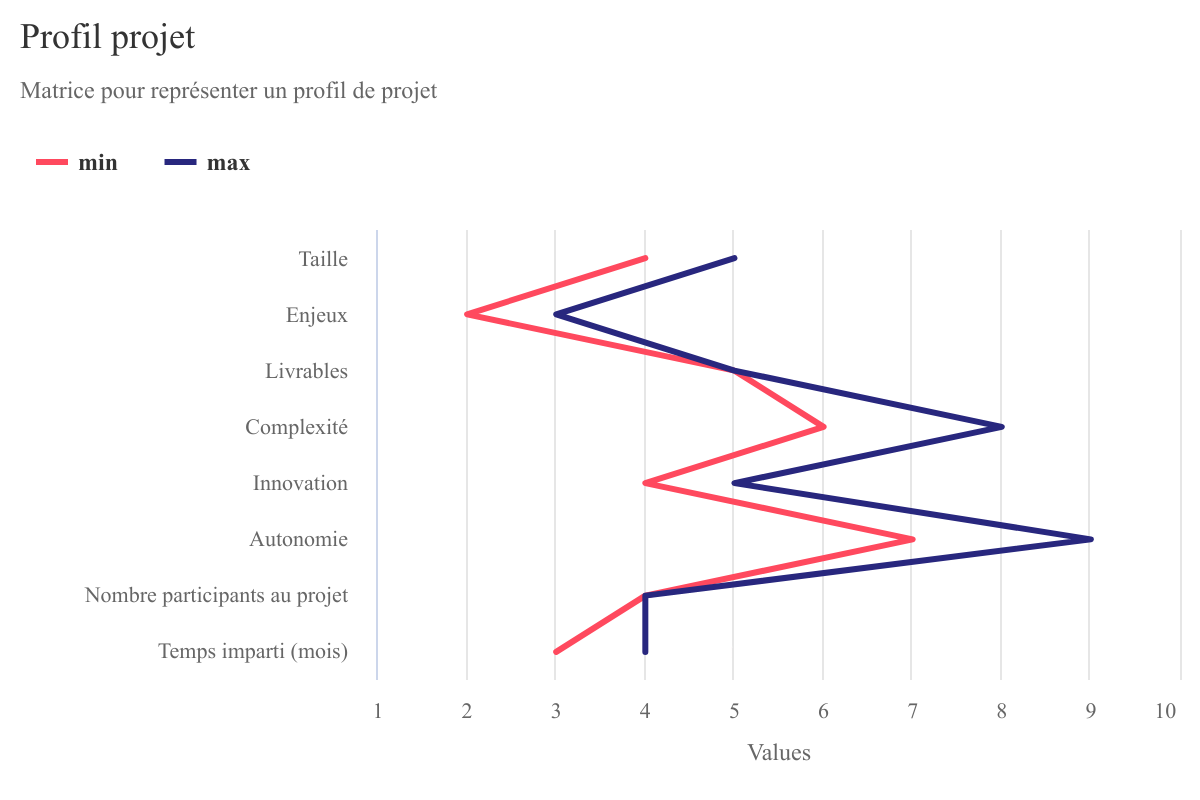
\includegraphics[width=0.75\textwidth]{img/profil_projet.png}
    \caption{Profil du projet}
\end{figure} 

\subsection{WBS : comment concrétiser l’application}
Ceci étant fait, nous avons maintenant choisi de détailler les lots de travail à effectuer pour fabriquer notre application. Nous avons ainsi réalisé le WBS de notre application : il apparait ainsi les grandes étapes de notre projet que sont : definition du cadre de l’application, développement des fonctionnalités de l’application et écriture du rapport.
\begin{figure}[H]
    \centering
    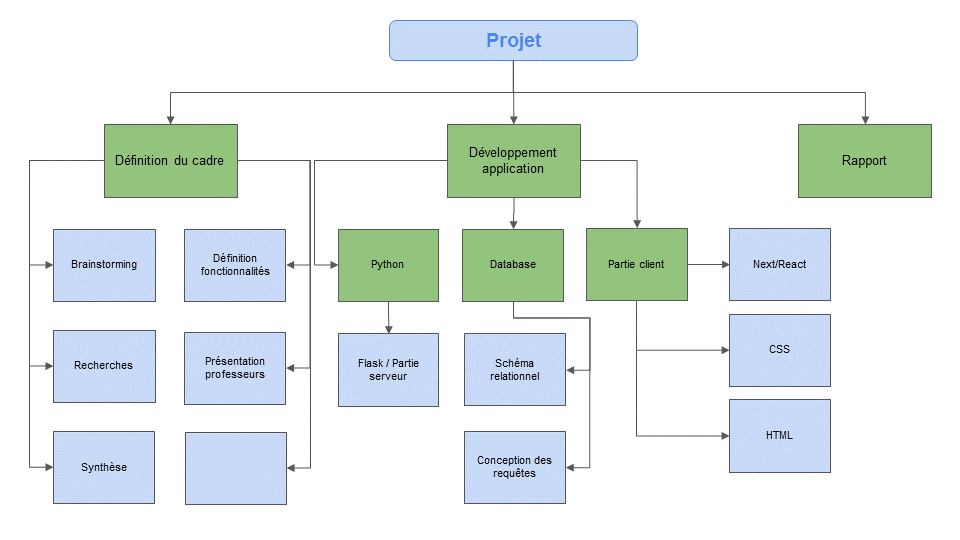
\includegraphics[width=0.75\textwidth]{img/WBS.png}
    \caption{WBS}
\end{figure} 

\subsection{Diagramme de Gantt : planification}
Maintenant que nous avons un détail des lots de travail qui constitue notre application, il faut maintenant les mettre en relation pour créer un planning efficace où chaque tâche est effectuée dans l’ordre.
\begin{figure}[H]
    \centering
    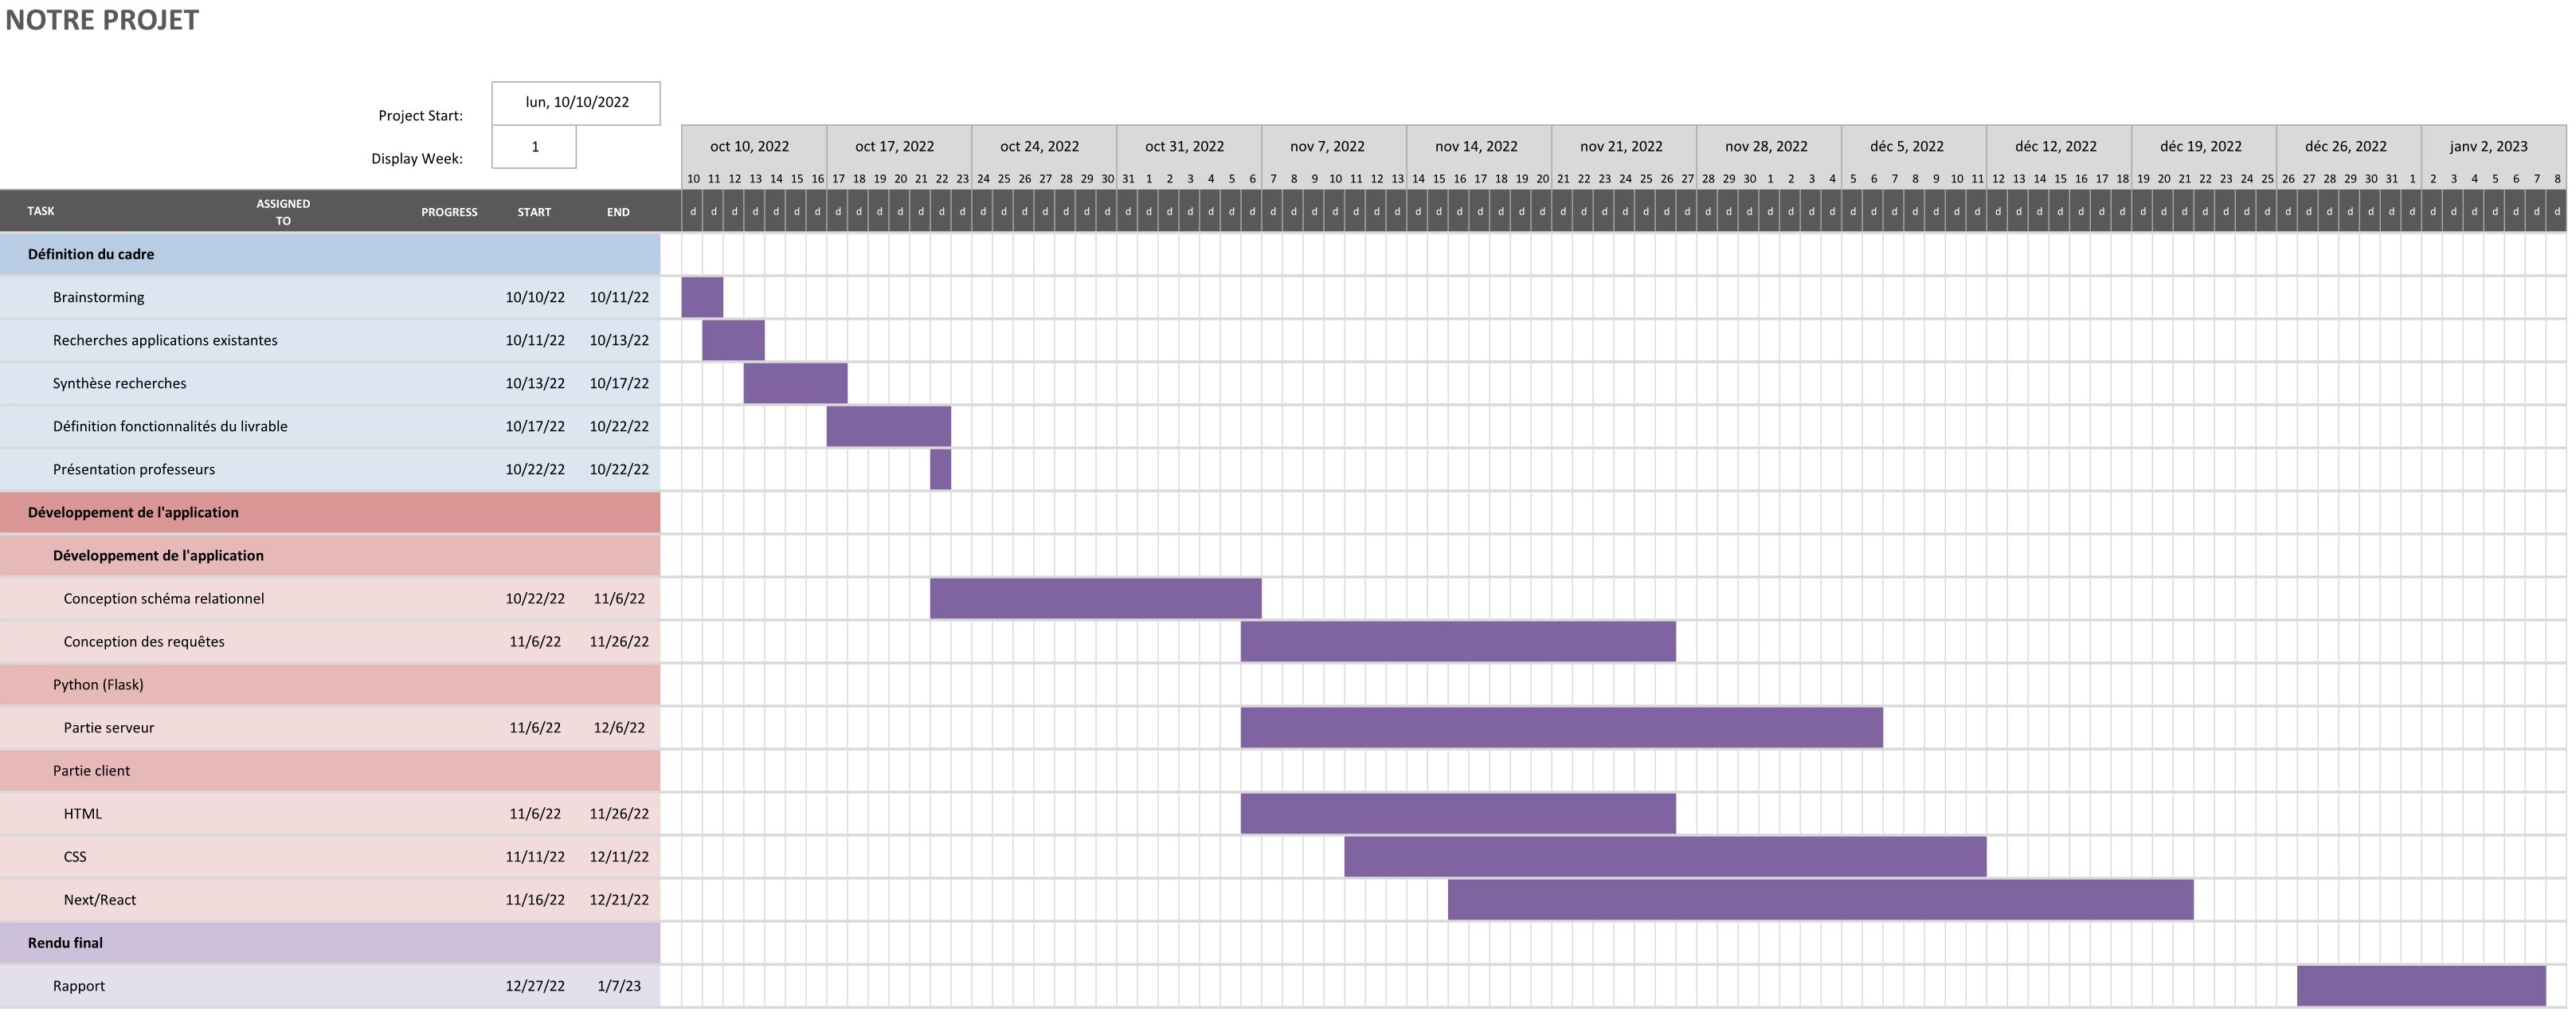
\includegraphics[width=0.9\textwidth]{img/gantt.jpeg}
    \caption{Diagramme de GANTT}
\end{figure} 
Il est clair que la partie conception doit précéder la partie programmation. La partie serveur, html, CSS étant effectué en parallèle.

\subsection{Matrice RACI}
Maintenant que toutes les étapes sont planifiées, il manque à répartir le travail entre les membres de l’équipe. On utilise ainsi une matrice RACI.
\begin{figure}[H]
    \centering
    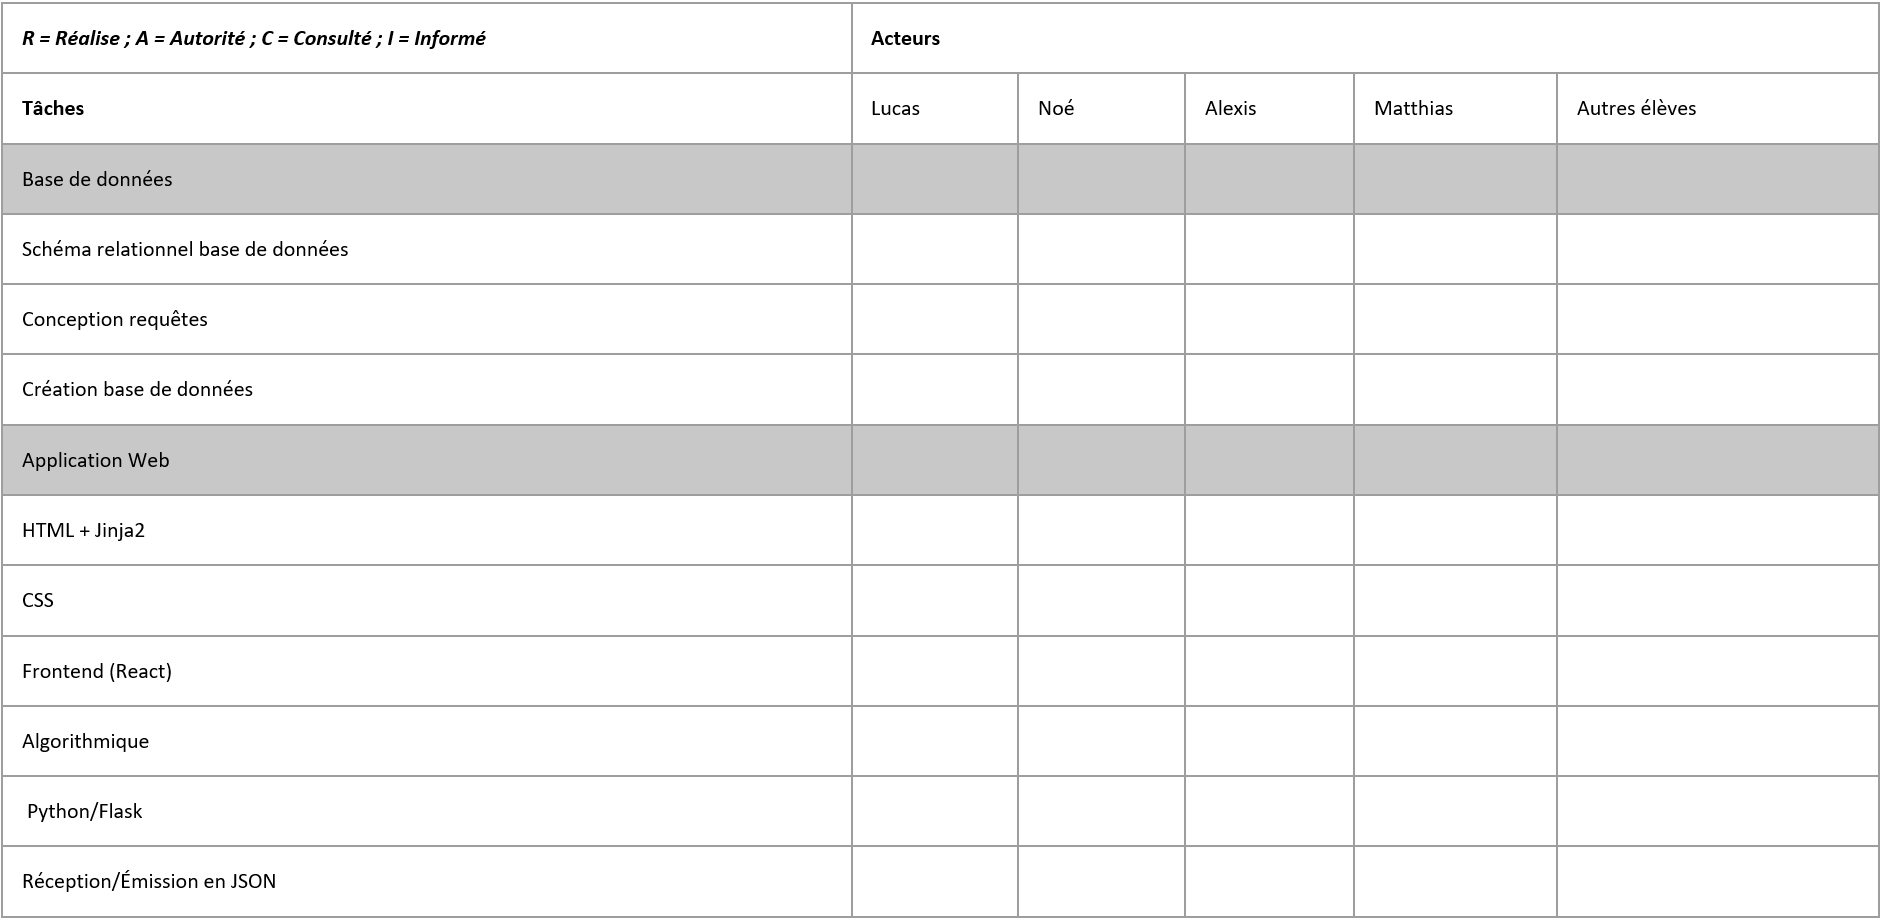
\includegraphics[width=0.75\textwidth]{img/RACI.png}
    \caption{Matrice RACI}
\end{figure} 

\newpage
\section{Application proposée}
\subsection{Définitions}
Idée générale : les jardins partagés / privés. Les jardins partagés sont des jardins gérés à plusieurs (une communauté, association de personnes), les terrains appartiennent à la commune dans lesquels ils se trouvent. Il faut s’inscrire sur les listes pour y accéder. Ils sont souvent liés à un quartier, il s’agit donc d’un environnement local. Ils permettent pour la plupart de cultiver des légumes, des fruits, des arbres fruitiers, des épices, du miel (avec des ruches). Ils ont pour vocation d’être des endroits conviviaux et orientés vers un certain respect de la nature (récupération de l’eau de la pluie, se soucier des produits utilisés, mettre en place des systèmes.
Les jardins privés, c’est la même chose, mais le terrain est géré par un particulier.
\subsection{Fonctionnalités de l'application}
\begin{itemize}
    \item Compte :
          \begin{itemize}
              \item Pour accéder aux fonctionnalités de l’application, une inscription sera nécessaire
          \end{itemize}
    \item Interactions d’un utilisateur avec les autres :
          \begin{itemize}
              \item créer un jardin :
                    \begin{itemize}
                        \item nom + adresse du jardin au minimum
                        \item deux états :
                              \begin{itemize}
                                  \item public : tout le monde peut voir le jardin sur la carte globale
                                  \item privé : seul les membres du jardin peuvent le voir sur la carte globale
                              \end{itemize}
                    \end{itemize}
              \item rejoindre un jardin :
                    \begin{itemize}
                        \item public : tout le monde peut directement faire une demande qui sera accepter ou non par le créateur du jardin
                        \item privé : un lien d’invitation envoyé par le créateur est nécessaire
                    \end{itemize}

          \end{itemize}
    \item fonctionnalités dans un jardin :
          \begin{itemize}
              \item création d’une modélisation du plan réel du jardin : création d’un jardin visuel suivant la forme du jardin réel
              \item  possibilité de diviser le jardin en plusieurs sous parties
              \item chaque partie du jardin a :
                    \begin{itemize}
                        \item état (labouré, semé : tomate, jachère…)
                        \item un liste des tâches à faire
                              \begin{itemize}
                                  \item intitulé de la tâche
                                  \item date limite de la tâche (optionnel)
                                  \item chaque tâche peuvent entre valider une fois faite
                              \end{itemize}
                        \item une historique des tâches qui ont été faite et par qui
                        \item possibilité de changer un état
                        \item possibilité d’ajouter,valider,supprimer des choses à faire
                    \end{itemize}
              \item vue global graphique des différents parties et états de chaque parties du jardin
          \end{itemize}
\end{itemize}
La création de la modélisation d’un jardin et de ses parties se fera de manière dynamique avec bloc graphique.

De même pour gérer l’état d’une partie, l’utilisateur pourra choisir le bloc qui correspond à son état et le glisser sur la partie du jardin correspondante.

\section{Conclusion}

\end{document}